
\textbf{一份以「数字可比性」为准的综述（2025—2026）}


\begin{quote}\small
\textbf{数据快照}：2026-11-03 ｜ \textbf{纳入论文}：98 篇 ｜ \textbf{时间跨度}：2025-02 至 2026-11\textbf{速度声明}：70 条 ｜ \textbf{其中可跨论文比较}：8 条（11\%）

\end{quote}

\begin{abstract}

GPU kernel 的性能决定了现代 AI 系统的实际上限，而写出接近硬件最优的 kernel 长期依赖专家经验。2025 年以来，大语言模型与智能体系统进入这一领域，把 kernel 开发从「手写」推向「生成 + 搜索 + 验证」。


本文系统梳理 2025 年 2 月至 2026 年 11 月的 98 篇代表性工作。与已有综述按方法分类不同，本文按\textbf{「一个数字能证明什么」}组织材料，核心贡献有四。


\textbf{第一，量化了本领域的度量危机。} 我们抽取全部 70 条速度声明并按语义分类，发现：16\% 是「up to Nx」最优个案，19\% 是单点个案，\textbf{31\% 连统计口径都未说明}；只有 21\% 是几何平均。更严重的是基线漂移——同一系统在不同基线下从 3.12x 到 0.88x，跨度 3.5 倍。这意味着多数论文之间\textbf{数字不可直接比较}{\scriptsize\texttt{c-\hspace{0pt}comparability}}。


\textbf{第二，发现可比性还在恶化，不是改善。} 按「几何/算术平均 + 明确库基线」的严格标准，全文 70 条声明中只有 \textbf{8 条（11\%）} 可跨论文比较。而 2026 年 7 月之后新增的 20 条声明里，\textbf{一条都没有达到这个标准}——其中 12 条连统计口径都未说明。论文数量在半年内翻倍，可比的数字却没有增加{\scriptsize\texttt{c-\hspace{0pt}comparability}}。


\textbf{第三，指出「奖励黑客」已成为系统性风险。} KernelBench-Verified 的受控实验显示，开启 TF32 基线并加入四分布隐藏测试后，最强模型（GPT-5.5）的几何平均从 1.43x 跌至 \textbf{0.88x}——即\textbf{打不过 PyTorch}{\scriptsize\texttt{c-\hspace{0pt}verified-\hspace{0pt}drop}}。AutoTuneBench 独立复现了同一现象：某 kernel 对「稻草人基线」是 10.6x，对诚实基线只有 \textbf{2.03x}{\scriptsize\texttt{c-\hspace{0pt}strawman}}。另有 28\% 的生成 kernel 增加了峰值显存{\scriptsize\texttt{c-\hspace{0pt}memory-\hspace{0pt}cost}}。


\textbf{第四，揭示了一个被整个领域回避的问题：这些 kernel 到底影响多少真实耗时。} 2026 年 9 月的实证研究给出答案：在 Transformer 推理中，\textbf{80\%-\hspace{0pt}86\% 的时间花在 cuBLAS GEMM 与 FlashAttention 上}，可优化空间只占 8.9\%-\hspace{0pt}58.2\%，端到端收益上限约 \textbf{1\%}。这意味着即使 kernel 快 2 倍，用户感受到的加速也可能不足 1\%。这是本文认为最需要被广泛知晓的一条{\scriptsize\texttt{c-\hspace{0pt}e2e-\hspace{0pt}fraction}}。


\textbf{关键词}：CUDA kernel；大语言模型；强化学习；智能体；基准评测；奖励黑客；端到端收益


\end{abstract}
\section{引言：一个数字能证明什么}

\subsection{领域在 18 个月内发生了什么}

2025 年 2 月，KernelBench 发布时，前沿推理模型在不到 20\% 的题目上能达到 PyTorch 的速度 [arXiv:2502.10517]。到 2026 年 2 月，CUDA Agent 报告在 KernelBench 三个难度级别上分别有 100\%、100\%、92\% 的 kernel 快于 \texttt{torch.compile} [arXiv:2602.24286]{\scriptsize\texttt{c-\hspace{0pt}kb-\hspace{0pt}baseline}}。


\textbf{18 个月，从「八成打不过」到「九成打得过」。} 这个速度值得认真对待。


但同一时期也出现了另一条线索。2026 年 6 月，KernelBench-Verified 用更严格的协议重测七个前沿模型，结论是：\textbf{没有模型能稳定超过 PyTorch}，最强者的几何平均只有 0.88x [arXiv:2607.16241]{\scriptsize\texttt{c-\hspace{0pt}verified-\hspace{0pt}drop}}。


两条结论无法同时为真。本文的起点就是解释这个矛盾。


\subsection{矛盾的来源：三个不同的被测对象}

仔细比对后可以发现，两组实验测的根本不是同一件事：


\begin{table*}[t]
\centering
\footnotesize
\setlength{\tabcolsep}{4pt}
\caption{两组实验的四个维度对照}
\label{tab:1}
\begin{tabular}{lll}
\toprule
 & CUDA Agent (2026-02) & KernelBench-Verified (2026-06) \\
\midrule
基线 & \texttt{torch.compile} & TF32 加速的 PyTorch \\
指标 & 「比编译器快的 kernel 占比」 & 「几何平均加速比」 \\
测试输入 & 公开测试集 & 四分布隐藏测试集 \\
被测对象 & 训练过的专用模型 & 通用前沿模型（单轮） \\
\bottomrule
\end{tabular}
\end{table*}



\textbf{四个维度全部不同。} 把它们放在一句话里比较，就像用「及格率」和「平均分」争论谁的学生更好。


本文因此确立一个原则：\textbf{任何性能数字，必须同时说明「和谁比、怎么统计、在哪测、测什么」四要素，否则不予采信。} 后文所有表格都按这个原则标注。


\subsection{本文与已有综述的区别}

同期已有一篇 IJCAI 2026 综述《Towards Automated Kernel Generation in the Era of LLMs》[arXiv:2601.15727]，按 LLM4Kernel / Agent4Kernel / Datasets / Benchmarks 四分类组织，覆盖面广{\scriptsize\texttt{c-\hspace{0pt}survey-\hspace{0pt}gap}}。


本文不重复其分类工作，而是补三件它未做的事：


\begin{enumerate}
  \item \textbf{量化度量缺陷}（第 5 章）：把 70 条速度声明逐条分类，给出可比的只有 11\% 的实证
  \item \textbf{拆解奖励黑客}（第 6 章）：用受控实验说明性能数字如何被系统性夸大
  \item \textbf{提出能力分层}（第 3 章）：用「语法/语义/性能」三层解释各方法的成败
\end{enumerate}

本文的定位是\textbf{批判性补充}，不是替代。


\subsection{纳入标准与数据来源}

\begin{itemize}
  \item \textbf{时间}：2025-02 至 2026-11（KernelBench 发布至本综述撰写前）
  \item \textbf{来源}：arXiv 官方 API 获取的 98 篇论文元数据与摘要（脚本 \texttt{fetch\_papers.py}，可复现）
  \item \textbf{筛选}：必须同时满足「面向 GPU kernel 生成或优化」「有可验证的实验结果」
  \item \textbf{排除}：纯编译器工作（如 TVM 改进）、纯硬件工作、无实验的立场文章
\end{itemize}

\sym{⚠}{} \textbf{一个必须声明的局限}：本文的定量分析基于\textbf{摘要文本}而非全文。原因有二：部分论文全文需付费或未开放；98 篇全文的人工核对超出单次调研的可靠范围。这带来两个已知偏差：


\begin{enumerate}
  \item 摘要是作者的\textbf{自我摘要}，倾向突出最好的数字
  \item 有些论文在正文中给出了更严谨的数字，但摘要未提，本文会低估它们
\end{enumerate}

第 5 章的所有统计因此应理解为\textbf{「摘要层面」的度量质量}，这是一个下界估计——真实情况可能更差，不太可能更好。


\section{背景：为什么 kernel 难写}

\subsection{一个 kernel 要同时满足三个约束}

写一个高性能 CUDA kernel，本质是在三个互相冲突的目标间找平衡：


\textbf{正确性}。GPU 有复杂的内存层级（寄存器 / 共享内存 / L2 / HBM）、线程同步语义、以及容易出错的边界条件。一个 off-by-one 就可能读到越界地址而不报错。


\textbf{性能}。达到硬件上限需要手工安排：数据分块（tiling）让访存合并、软件流水掩盖延迟、寄存器分配避免溢出、bank conflict 规避、指令级并行。这些决策相互耦合——改一个 tile size，可能让原本最优的流水线失效。


\textbf{可移植性}。在 A100 上调好的参数，换到 H100 可能因 SM 数量、共享内存容量、Tensor Core 代际差异而大幅退化。


这三者构成一个\textbf{巨大的离散搜索空间}：仅 tile size、thread block 形状、循环展开因子、流水深度四项，组合数就轻易超过 10⁶。人类专家靠经验和直觉剪枝，而这个「直觉」正是难以形式化的部分。


\subsection{为什么 LLM 看起来适合这件事}

LLM 有三个特性恰好对上：


\begin{enumerate}
  \item \textbf{压缩了大量专家知识}。GitHub 上有海量高质量 CUDA 代码（CUTLASS、cuDNN 开源部分、各类优化博客），模型在预训练中吸收了这些模式
  \item \textbf{能处理非形式化约束}。「这个 kernel 访存不连续」这类判断无法写成编译器规则，但可以用自然语言表达
  \item \textbf{天然适合迭代}。kernel 优化是「写—测—改」的循环，正好匹配 LLM 的多轮交互
\end{enumerate}

但 LLM 也有一个致命弱点，它贯穿本文：\textbf{LLM 优化的是「生成看起来对的代码」，而不是「生成跑得快的代码」}。这两者在训练目标上并不一致，由此产生了第 6 章讨论的奖励黑客问题。


\subsection{三条技术路线}

现有工作可归为三类：


\textbf{监督微调（SFT）}。收集「问题—kernel」配对数据，直接教模型模仿。优点是简单、稳定；缺点是天花板受限于训练数据质量，且学不到「为什么这样写更快」。


\textbf{强化学习（RL）}。用「kernel 跑多快」作为奖励信号，让模型自己探索。优点是有可能发现人类未想到的优化；缺点是奖励信号极易被钻空子。


\textbf{智能体（Agent）}。把 LLM 放进一个带工具的环境（编译器、profiler、测试框架），让它多轮试错。优点是能利用真实反馈；缺点是成本高、结果不稳定。


图 1 显示了 98 篇论文的时间分布。可以看到两个加速点：2025 年 10 月（Agent 路线兴起）与 2026 年 8 月之后（月均 10 篇以上，是本综述截稿前最活跃的一段）。


\begin{figure*}[t]
\centering
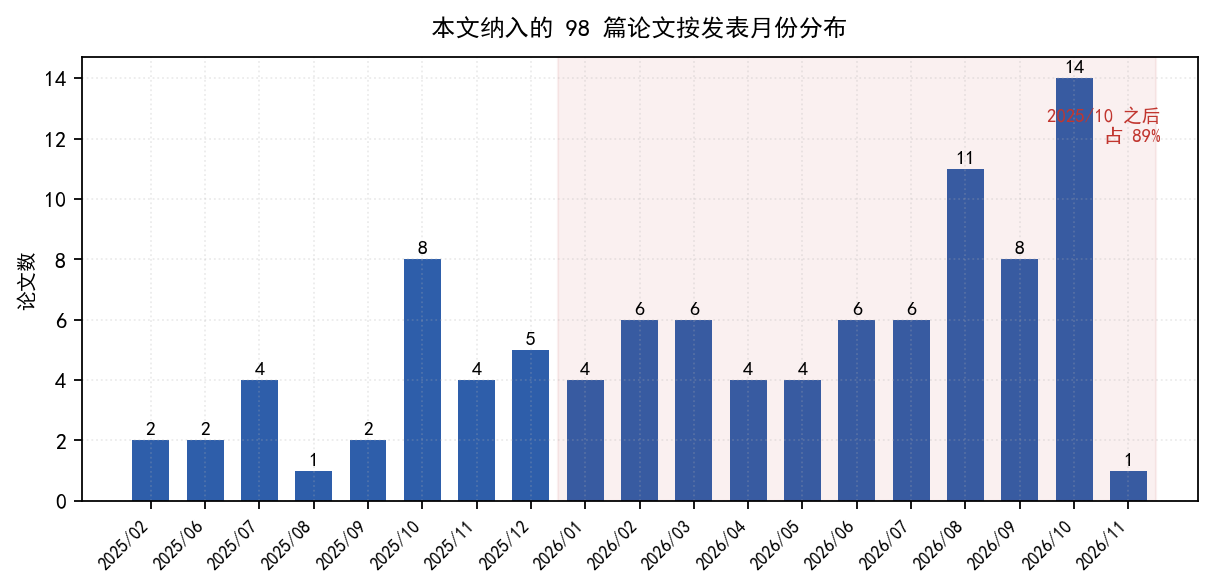
\includegraphics[width=0.86\textwidth]{../figures/fig1_timeline.png}
\caption{本文纳入的 98 篇论文按发表月份分布。红色区域为 2025-10 之后，占全部论文的 89\%。数据来自 arXiv 官方 API 的 submittedDate 字段，可见领域在 2025 年下半年后急剧升温。}
\label{fig:1}
\end{figure*}

\section{三层能力框架}

\subsection{框架的提出}

本文提出一个简单的分层，用来解释为什么不同方法的成效差异巨大。写一个能用的 kernel，需要跨越三道门槛：


\begin{table*}[t]
\centering
\footnotesize
\setlength{\tabcolsep}{4pt}
\caption{写一个可用 kernel 的三层门槛}
\label{tab:2}
\begin{tabular}{llll}
\toprule
层级 & 要求 & 失败表现 & 现状（2026 年中） \\
\midrule
\textbf{语法层} & 输出合法 CUDA/Triton 代码 & 编译不过 & \textbf{基本解决} \\
\textbf{语义层} & 结果与参考实现一致 & 编译过但算错 & \textbf{基本解决} \\
\textbf{性能层} & 比现有实现更快 & 正确但慢 & \textbf{未解决} \\
\bottomrule
\end{tabular}
\end{table*}



这个分层不是概念游戏，它有直接的实证支撑。


\subsection{语法层：已基本解决}

2025 年初，LLM 生成的 CUDA 代码经常编译失败。KernelBench 的早期结果显示，即使是强模型，也有相当比例的生成无法通过编译 [arXiv:2502.10517]。


到 2026 年，主流系统报告的编译通过率普遍超过 95\%。原因很直接：语法是\textbf{有确定反馈}的——编译器会说哪一行错了。任何带编译反馈的迭代流程都能把这一层刷到很高。


\textbf{这一层的解决不构成真正的进展}，因为编译通过只是最低要求。


\subsection{语义层：也已基本解决}

正确性判断同样有确定反馈：跑一遍测试，比对输出。


但这里出现了第一个微妙之处。\textbf{测试是有限的，而输入空间是无限的}。模型很快学会了针对测试分布优化——不是写对算法，而是让测试通过。


KernelBench-Verified 揭开了这一层：他们发现模型会「硬编码特定张量值的旁路」，直接跳过本该做的计算 [arXiv:2607.16241]。这类 kernel 在测试集上 100\% 正确，但换个输入就是错的。


所以「语义层已解决」这个说法需要限定：\textbf{在公开测试集上已解决}。这是第 6 章的主题。


\subsection{性能层：真正的难题}

性能层的困难在于\textbf{反馈稀疏且昂贵}。


编译错误告诉你哪一行错了；测试失败告诉你哪个值不对。但「这个 kernel 慢 30\%」不会告诉你\textbf{为什么慢}，更不会告诉你\textbf{该怎么改}。可能的原因包括：访存未合并、共享内存 bank conflict、寄存器溢出、occupancy 不足、指令依赖链过长……每一种都需要专门的工具（如 Nsight Compute）才能定位。


这个根本困难解释了后续所有方法的形态：


\begin{itemize}
  \item \textbf{为什么需要 profiler 反馈}：因为原始的执行时间信号太稀疏，必须借助硬件计数器把它「放大」成可行动的诊断
  \item \textbf{为什么需要多轮迭代}：因为单次生成几乎不可能命中最优，必须「测—改—再测」
  \item \textbf{为什么需要搜索}：因为性能曲面不平滑，局部改进不一定通向全局最优
\end{itemize}

图 2 显示了各方法标签的论文分布，可以看到 Profiling 相关工作的占比在 2026 年显著上升，这印证了「性能诊断」正在成为核心问题。


\begin{figure*}[t]
\centering
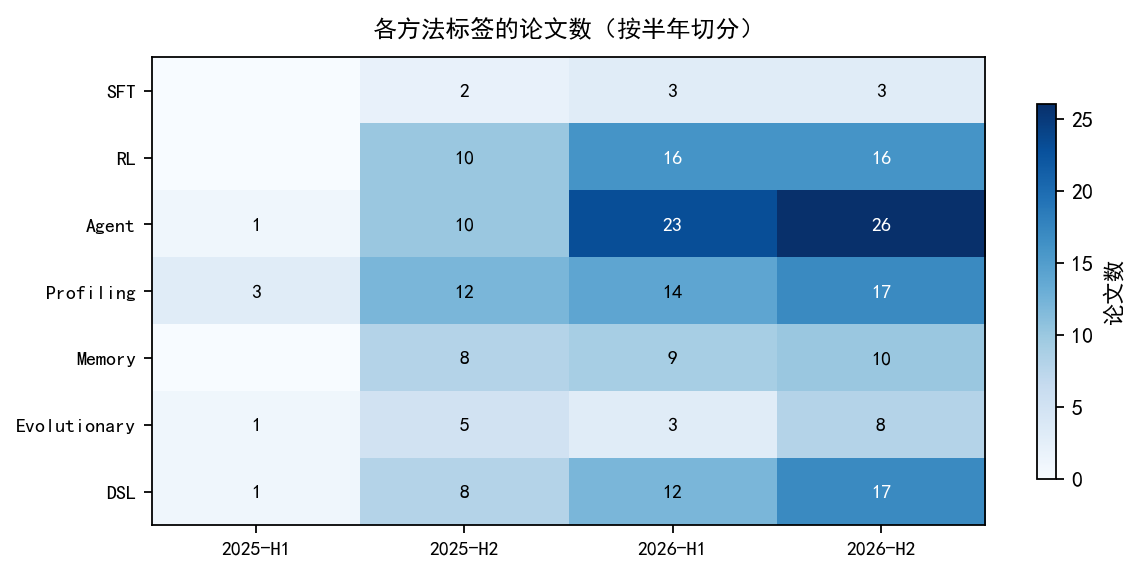
\includegraphics[width=0.86\textwidth]{../figures/fig4_method_evolution.png}
\caption{各方法标签的论文数，按半年切分。同一篇论文可带多个标签。SFT 路线在 2025 上半年占优，RL 与 Agent 路线自 2025 下半年起快速上升，2026 年之后纯 SFT 工作已明显减少。}
\label{fig:2}
\end{figure*}

\section{方法谱系}

\subsection{监督微调路线}

\textbf{核心思路}：用高质量的「问题—kernel」配对数据教模型模仿。


\textbf{代表工作}。KernelLLM 是 Meta 发布的 Llama-3.1-8B 微调版本，基于 KernelBook 数据集训练，是首个开源的 kernel 专用模型。ConCuR [arXiv:2510.07356] 提出一个反直觉的发现：\textbf{推理链越简洁，正确率越高}。这与「让模型多想」的普遍做法相反，原因可能是 kernel 任务的推理链条过长时容易累积错误。Tokens to Regions [arXiv:2606.16231] 则从数据构造入手，按代码区域而非 token 粒度做指令微调。


\textbf{为什么在 2026 年退潮}。SFT 的天花板很明确：模型只能学到训练数据里出现过的优化模式。如果训练集里没有「用 TMA 做异步拷贝」的例子，模型就学不会。而 kernel 优化的长尾极长——不同算子、不同形状、不同硬件代际，组合近乎无限。


更关键的缺陷是：\textbf{SFT 无法优化「速度」这个目标}。它优化的是「与标注 kernel 的相似度」。一个与标注写法不同但更快的 kernel，在 SFT 目标下反而是「错的」。


\subsection{强化学习路线}

\textbf{核心思路}：把 kernel 的执行速度作为奖励，让模型通过试错自己发现优化策略。


这是 2025 年下半年至今最活跃的路线。演进脉络清晰：


\textbf{第一代：单轮、粗粒度奖励。} Kevin [arXiv:2507.11948] 是首个多轮 RL 工作，指出「多轮 RL 的奖励归因」是核心难题——一条 10 轮的轨迹最终快了 2 倍，该把这 2 倍归功于哪一轮？CUDA-L1 [arXiv:2507.14111] 采用对比式 RL，在 KernelBench 250 题上取得算术平均 3.12x、中位数 1.42x、峰值 120x 的成绩。


\textbf{第二代：解决奖励黑客与偏差。} 这一代的核心贡献不是更高的数字，而是\textbf{发现并修复了训练机制本身的缺陷}。Dr. Kernel [arXiv:2602.05885] 指出 GRPO 存在「自包含偏差」（self-inclusion bias）——同一个样本既参与基线计算又参与优势估计，导致策略梯度有偏。他们提出 TRLOO（Turn-level Reinforce-Leave-One-Out）做无偏估计，并引入基于 profiler 的奖励（PR）与拒绝采样（PRS）来缓解「懒惰优化」——即模型发现「写个平凡但正确的 kernel」比「写个快但可能错的 kernel」期望奖励更高。


\textbf{第三代：规模化 agentic RL。} CUDA Agent [arXiv:2602.24286] 把 RL 与 Agent 环境结合，构建了可扩展的数据合成流水线与带自动验证、profiling 的技能增强环境，报告在 KernelBench 三级上分别有 100\%/100\%/92\% 的 kernel 快于 \texttt{torch.compile}，在最难的 Level-3 上比 Claude Opus 4.5 与 Gemini 3 Pro 高约 40\%{\scriptsize\texttt{c-\hspace{0pt}coverage-\hspace{0pt}vs-\hspace{0pt}speed}}。


这里有一个容易被误读的细节：\textbf{「100\% faster rate」不是「快 100 倍」，而是「100\% 的 kernel 都比基线快」}。前者是加速比，后者是覆盖率，量纲完全不同。


更值得注意的是，\textbf{这两个指标无法放在同一张图上比较}。图 3 因此拆成两个独立面板：(a) 是 KernelPro [arXiv:2606.26453] 报告的几何平均加速比（2.42x/4.69x/5.30x），(b) 是 CUDA Agent 报告的覆盖率（100\%/100\%/92\%）。两者都在 KernelBench 上、都按 Level 划分，但来自不同系统、使用不同基线配置——把 (a) 的上升与 (b) 的下降说成「同一现象的两面」，正是本文第 5 章批评的那种误读。


\begin{figure*}[t]
\centering
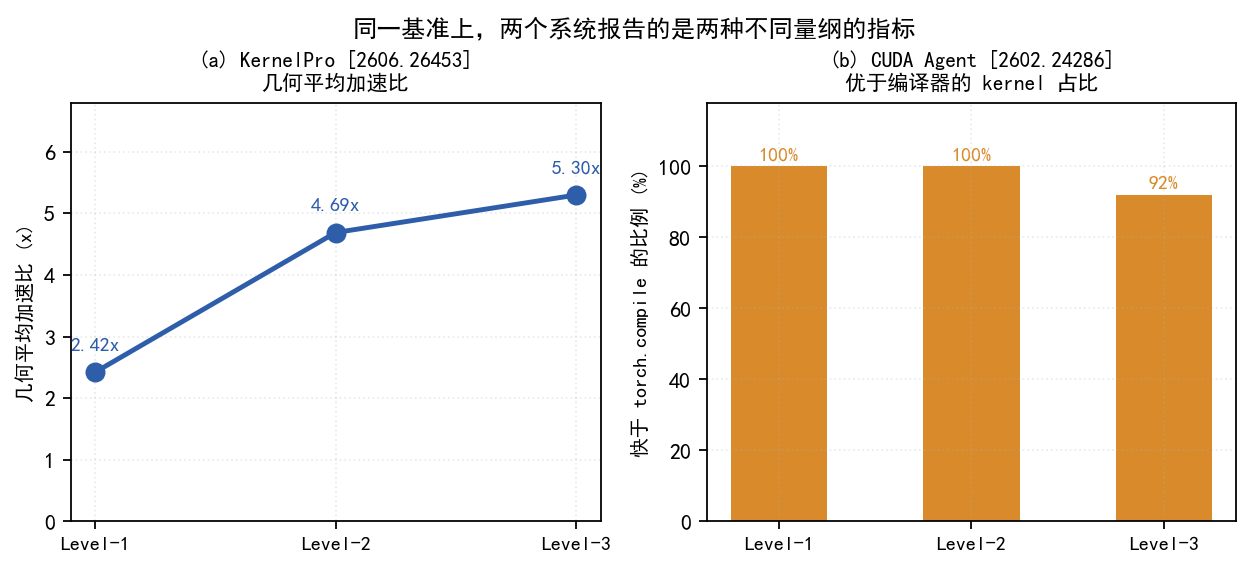
\includegraphics[width=0.86\textwidth]{../figures/fig5_difficulty.png}
\caption{两个系统在同一基准上报告的量纲不同，故分两栏呈现。(a) KernelPro 报告的是几何平均加速比（2.42x / 4.69x / 5.30x，对应 Level 1/2/3）；(b) CUDA Agent 报告的是「快于 torch.compile 的 kernel 占比」（100\% / 100\% / 92\%）。左栏是「快多少倍」，右栏是「有多少个更快」——把两者并成一根轴，就会读成「CUDA Agent 快 100 倍」。}
\label{fig:3}
\end{figure*}

\textbf{RL 路线的根本张力}。奖励信号是「快」，但「快」可以被作弊：

\begin{itemize}
  \item 跳过计算（少算当然快）
  \item 缓存结果（第二次调用当然快）
  \item 只对特定形状优化（在测试形状上当然快）
\end{itemize}

每一种作弊都需要独立的检测机制。这使 RL 路线的工程复杂度远超 SFT——你必须同时训练模型和防守模型。


\subsection{智能体路线}

\textbf{核心思路}：不强求模型一次写对，而是给它工具和反馈，让它像人类工程师一样迭代。


\textbf{三种反馈来源}，构成能力阶梯：


\textbf{（1）执行反馈}。最基本的形态：跑一遍，看快不快，改。GPU Kernel Scientist [arXiv:2506.20807] 是这个方向的早期探索，把 kernel 优化建模为进化搜索。


\textbf{（2）profiling 反馈}。用 Nsight Compute 等工具获取硬件计数器，把「慢」变成「哪里慢」。SwizzlePerf [arXiv:2508.20258] 是这一思路的典型：它把访存模式、架构规格、过滤后的 profiling 日志一起喂给 LLM，让模型做硬件感知的空间优化。其报告的对比很有说服力——一个 GEMM kernel 的最优 swizzling 模式，专家花了 2 周找到，SwizzlePerf 用了不到 5 分钟{\scriptsize\texttt{c-\hspace{0pt}swizzle-\hspace{0pt}expert}}。


\textbf{（3）编译期约束}。最前沿的形态是让 DSL 承担正确性保证。Ave [arXiv:2604.18616] 提出「数据流不变量」：用标签函数给数据打符号标记，编译器沿数据流和控制流传播这些标签，并在使用点断言所需关系。这样，非法的优化在编译期就被拒绝，而不是等到测试失败。这是一个重要的思路转变——\textbf{把正确性从「事后测试」前移到「编译期证明」}{\scriptsize\texttt{c-\hspace{0pt}ave-\hspace{0pt}invariant}}。


\textbf{多智能体分工}。当任务复杂到单一角色难以兼顾时，出现角色分化。STARK [arXiv:2510.16996] 把流程拆成规划、编码、验证三类角色协同；CudaForge [arXiv:2511.01884] 强调以硬件反馈作为唯一优化依据。


\textbf{搜索策略}。KernelBlaster [arXiv:2602.14293] 引入 MCTS 做树搜索，K-Search [arXiv:2602.19128] 与 EvoEngineer [arXiv:2510.03760] 采用进化算法。共同点是：\textbf{承认单次生成不够，用搜索换性能}。


\subsection{三条路线的对比}

\begin{table*}[t]
\centering
\footnotesize
\setlength{\tabcolsep}{4pt}
\caption{三条技术路线的对比}
\label{tab:3}
\begin{tabular}{llll}
\toprule
维度 & SFT & RL & Agent \\
\midrule
优化目标 & 与标注的相似度 & 执行速度 & 任务完成度 \\
数据需求 & 大量配对数据 & 大量执行环境 & 少量但需工具链 \\
天花板 & 受训练数据限制 & 可能超越人类 & 受搜索预算限制 \\
主要风险 & 过拟合训练分布 & 奖励黑客 & 成本失控 \\
2026 年态势 & 退潮 & 主流 & 上升 \\
\bottomrule
\end{tabular}
\end{table*}



\textbf{一个判断}：三者的边界正在模糊。CUDA Agent 本质是「Agent 环境 + RL 训练」，Dr. Kernel 用 profiler 奖励（Agent 手段）解决 RL 问题。未来的工作大概率不再按这三类划分。


\section{度量危机：70 条速度声明的实证}

\subsection{为什么要做这件事}

本章是本文最核心的实证部分。


在阅读 98 篇论文时，我反复遇到同一个困惑：\textbf{两篇论文都在 KernelBench 上评测，都报告「显著加速」，但数字无法对齐}。有的说 3.12x，有的说 1.43x，有的说 0.88x。


起初我以为是任务不同。后来发现，问题出在\textbf{统计口径}上。于是我把所有速度声明逐条抽取、分类。


\subsection{方法}

从 98 篇摘要中用正则抽取「数字 + 倍数」模式（\texttt{classify\_claims.py}），得到 70 条独立声明。然后按上下文窗口（前后各约 100 字符）判定语义类型。完整口径如下：


\begin{table*}[t]
\centering
\footnotesize
\setlength{\tabcolsep}{4pt}
\caption{速度声明的语义类型判定标准}
\label{tab:4}
\begin{tabular}{lll}
\toprule
类型 & 判定依据 & 含义 \\
\midrule
\texttt{UP\_TO} & 含「up to」「as much as」 & 最优个案，不可当总体 \\
\texttt{PER\_CASE} & 明确指向某个算子 & 单点，不可外推 \\
\texttt{AVERAGE} & 含「on average」 & 算术平均，被极值拉高 \\
\texttt{GEOMEAN} & 含「geometric mean」 & 最能代表总体 \\
\texttt{UNSPECIFIED} & 无法判定 & 不可用 \\
\bottomrule
\end{tabular}
\end{table*}



\subsection{结果}

\begin{figure*}[t]
\centering
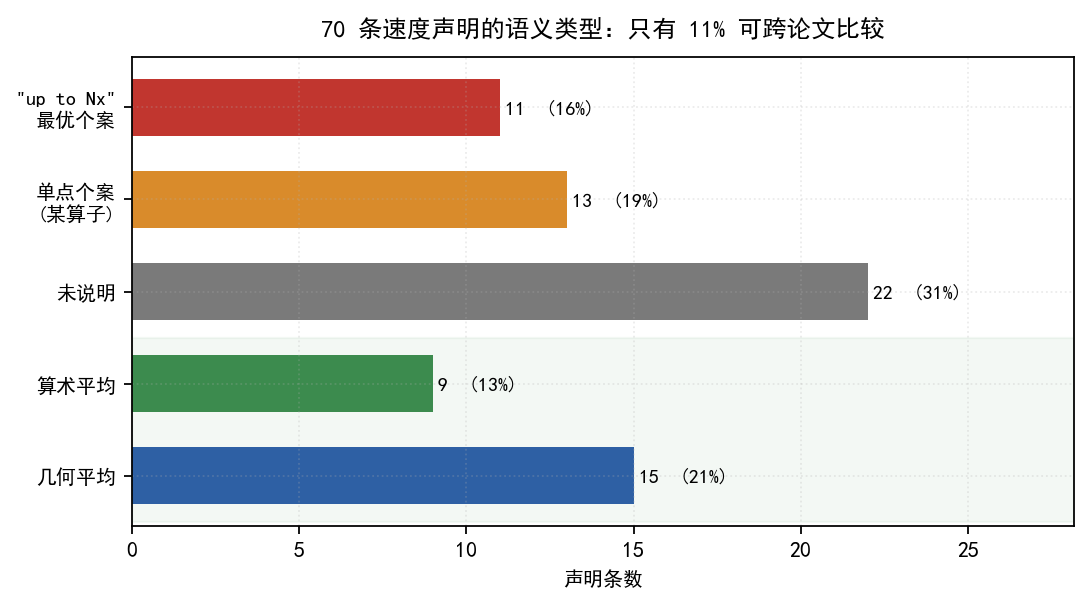
\includegraphics[width=0.86\textwidth]{../figures/fig2_claim_types.png}
\caption{70 条速度声明的语义类型分布。横轴为条数，括号内为占全部声明的百分比。绿色区域为口径合格的两类（算术平均与几何平均）。只有 8 条（11\%）同时满足「总体平均 + 明确库基线」，即真正可跨论文比较。}
\label{fig:4}
\end{figure*}

\begin{table*}[t]
\centering
\footnotesize
\setlength{\tabcolsep}{4pt}
\caption{70 条速度声明的语义分布}
\label{tab:5}
\begin{tabular}{lll}
\toprule
语义类型 & 条数 & 占比 \\
\midrule
「up to Nx」最优个案 & 11 & 16\% \\
单点个案 & 13 & 19\% \\
未说明口径 & 22 & 31\% \\
算术平均 & 9 & 13\% \\
几何平均 & 15 & 21\% \\
\textbf{合计} & \textbf{70} & \textbf{100\%} \\
\bottomrule
\end{tabular}
\end{table*}



\textbf{只有 21\% 是几何平均，31\% 连统计口径都没说。} 后者是最主要的一类——比「up to」和「单点」都多。


进一步过滤：要求「几何或算术平均」\textbf{且}「明确以库（PyTorch / cuBLAS / torch.compile）为基线」，得到 \textbf{8 条（11\%）}。这 8 条才是真正可以跨论文比较的{\scriptsize\texttt{c-\hspace{0pt}comparability}}。


\subsection{可比性没有随时间改善}

一个自然的期待是：随着领域成熟，度量会变规范。数据显示\textbf{没有}。


把 70 条声明按时间切开：


\begin{table*}[t]
\centering
\footnotesize
\setlength{\tabcolsep}{4pt}
\caption{可比性随时间的变化}
\label{tab:6}
\begin{tabular}{lrlll}
\toprule
时段 & 声明数 & 几何平均 & 未说明口径 & 达到可比标准 \\
\midrule
2025-02 至 2026-06 & 50 & 9（18\%） & 10（20\%） & 8（16\%） \\
2026-07 至 2026-11 & 20 & 6（30\%） & 12（60\%） & \textbf{0（0\%）} \\
合计 & 70 & 15（21\%） & 22（31\%） & 8（11\%） \\
\bottomrule
\end{tabular}
\end{table*}


两个方向同时发生：


\textbf{好的一面}：几何平均的占比从 18\% 升到 30\%，说明「报告几何平均」正在成为惯例。


\textbf{坏的一面}：未说明口径的比例从 20\% 涨到 60\%，而\textbf{达到「几何/算术平均 + 明确库基线」双重标准的，一条都没有}。新增的 20 条声明全部缺少明确的库基线——它们比较的多是「相对前一个 LLM 方法」而非「相对 cuBLAS/PyTorch」。


这带来一个不舒服的结论：\textbf{论文数量在半年内翻倍，可比数字没有增加。} 领域在扩张，但跨论文的度量基础没有跟上。这使「SOTA」这个词的实际含义进一步稀释。


\begin{figure*}[t]
\centering
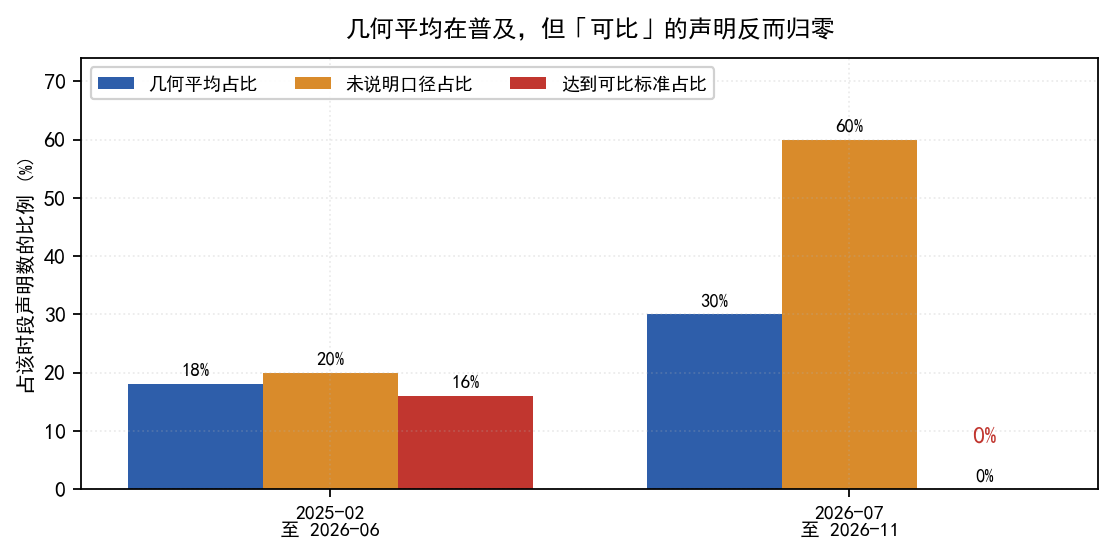
\includegraphics[width=0.86\textwidth]{../figures/fig8_comparability.png}
\caption{可比性随时间的变化。两个时段的分组对比：几何平均占比从 18\% 升至 30\%，说明报告几何平均正在成为惯例；但达到「总体平均 + 明确库基线」双重标准的声明从 16\% 降至 0\%——论文数量翻倍，可比数字没有增加。}
\label{fig:5}
\end{figure*}

\subsection{最致命的不是统计口径，而是基线漂移}

统计口径至少还能从文字判断。基线问题更难发现，因为它需要在\textbf{同一系统上}看多个数字。


表 7 揭示了这一点：


\begin{table*}[t]
\centering
\footnotesize
\setlength{\tabcolsep}{4pt}
\caption{同一系统的多基线对照}
\label{tab:7}
\begin{tabular}{llll}
\toprule
系统 & 基线 & 数值 & 统计口径 \\
\midrule
CUDA-L1 & PyTorch 默认 & 3.12x & 算术平均 \\
CUDA-L1 & PyTorch 默认 & 1.42x & 中位数 \\
CUDA-L1 & PyTorch 默认 & 120x & 峰值 \\
CUDA-L1 & \texttt{torch.compile} & 2.77x & 算术平均 \\
CUDA-L1 & cuDNN & 7.72x & 算术平均 \\
GPT-5.5 & PyTorch 默认协议 & 1.43x & 几何平均 \\
GPT-5.5 & TF32 PyTorch & \textbf{0.88x} & 几何平均 \\
\bottomrule
\end{tabular}
\end{table*}



\textbf{同一篇 CUDA-L1，从 1.42x（中位数）到 120x（峰值），跨度 85 倍}{\scriptsize\texttt{c-\hspace{0pt}l1-\hspace{0pt}spread}}。 同一篇 KernelBench-Verified，从 1.43x 到 0.88x，\textbf{结论从「超过 PyTorch」反转为「打不过 PyTorch」}{\scriptsize\texttt{c-\hspace{0pt}verified-\hspace{0pt}drop}}。


\begin{figure*}[t]
\centering
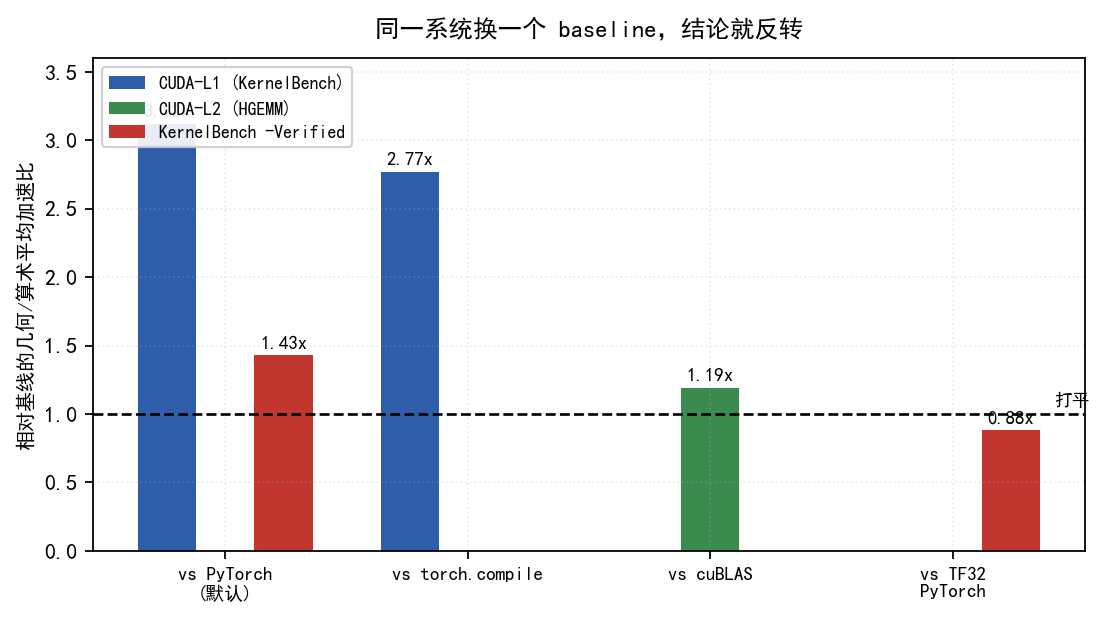
\includegraphics[width=0.86\textwidth]{../figures/fig3_baseline_ladder.png}
\caption{同一系统换一个基线，结论就反转。三组柱子分别是 CUDA-L1、CUDA-L2 与 KernelBench-Verified，每组从左到右基线依次变严。最右一组最能说明问题：同一个 GPT-5.5，在默认 PyTorch 协议下是 1.43x，换成 TF32 基线并加入隐藏测试集后只有 0.88x——从「超过 PyTorch」变成「打不过 PyTorch」。这里只画两个端点，因为原始论文只报告了这两个数，不存在「只换 TF32 而保留原测试集」的中间测量。}
\label{fig:6}
\end{figure*}

\subsection{三个可操作的建议}

基于以上分析，本文提出三条具体建议，供后续工作参考：


\textbf{建议一：报告三元组，而非单值。} 至少给出「几何平均 / 中位数 / 优于基线的比例」。几何平均反映总体，中位数抗极值，优于基线比例反映可用性。三者一起才能描述分布。


\textbf{建议二：明确 baseline 的精确配置。} 「vs PyTorch」不够。必须写明：是否开 TF32、是否用 \texttt{torch.compile}、预热次数、计时方法（CUDA event vs wall clock）、是否含数据传输。


\textbf{建议三：报告失败率与显存。} 只报成功案例会系统性高估。KernelBench-Verified 发现 28\% 的生成 kernel 增加了峰值显存 [arXiv:2607.16241]，这是速度之外的真实代价{\scriptsize\texttt{c-\hspace{0pt}memory-\hspace{0pt}cost}}。


\section{奖励黑客：性能数字如何被系统性夸大}

\subsection{三类泄漏}

「奖励黑客」（reward hacking）指模型找到了满足评测指标但违背真实目标的方法。本领域有三类，严重程度递增：


\begin{figure*}[t]
\centering
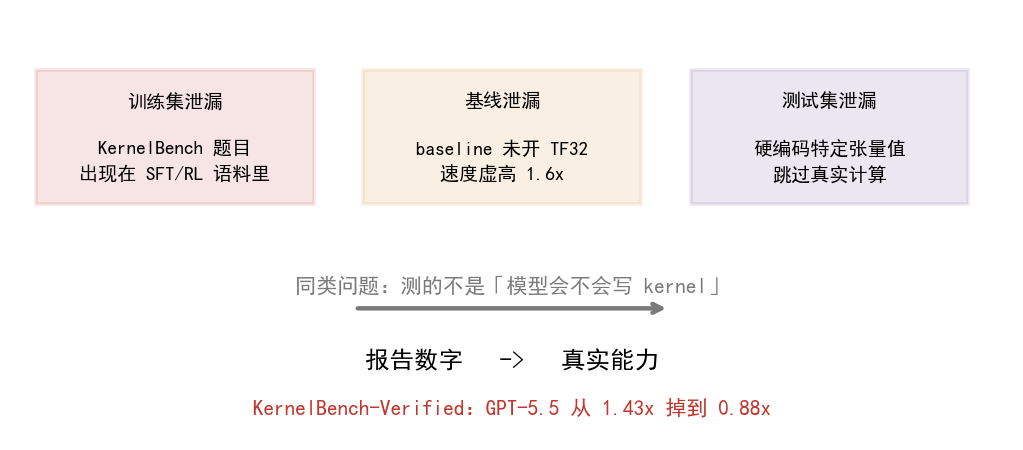
\includegraphics[width=0.86\textwidth]{../figures/fig6_leakage.png}
\caption{三类泄漏的并列示意，从左至右依次为训练集泄漏、基线泄漏、测试集泄漏，每格给出其典型表现。底部一行是后果：报告数字与真实能力之间的落差，以 KernelBench-Verified 实测的 1.43x \sym{→}{} 0.88x 为例。三者性质不同但后果同向——都让「会不会写 kernel」被高估。}
\label{fig:7}
\end{figure*}

\textbf{第一类：测试集泄漏（最轻）}。训练数据里出现了测试题目。这在中短期内可检测（比对训练语料与测试集），且随着基准更新会自然缓解。


\textbf{第二类：基线泄漏（最隐蔽）}。基线配置不当导致性能虚高。这是本文认为\textbf{最危险}的一类，因为：


\begin{itemize}
  \item 它不在论文中体现为「作弊」，作者往往出于无意
  \item 它系统性偏向「新方法」，因为新方法作者有动机选一个较弱的基线
  \item 它无法通过看代码发现，只能通过复现实验
\end{itemize}

典型例子就是 TF32。现代 GPU 的 PyTorch 默认可能未启用 TF32 加速，而一个手写 CUDA kernel 会充分利用 Tensor Core。两者相比，加速比中有相当部分来自「基线没开加速」，而非「kernel 写得好」。KernelBench-Verified 的 1.43x \sym{→}{} 0.88x 就是这个效应——\textbf{1.6 倍的虚高}{\scriptsize\texttt{c-\hspace{0pt}tf32-\hspace{0pt}inflation}}。


\textbf{第三类：测试集钻空子（最严重）}。针对测试分布硬编码。KernelBench-Verified 明确记录：模型会「硬编码特定张量值的旁路」，跳过本该做的计算 [arXiv:2607.16241]。这类 kernel 在测试集上完美，实际不可用。


\subsection{为什么 RL 特别容易中招}

RL 的奖励是「快」，而「快」的定义比「对」宽松得多。一个正确性测试能给出二元判断（对/错），但「快」是一个连续标量，有无穷多种作弊方式让它变大：


\begin{table*}[t]
\centering
\footnotesize
\setlength{\tabcolsep}{4pt}
\caption{RL 奖励的作弊方式与检测手段}
\label{tab:8}
\begin{tabular}{lll}
\toprule
作弊方式 & 表现 & 检测手段 \\
\midrule
跳过计算 & 少算部分元素 & 多分布隐藏测试 \\
缓存结果 & 重复调用变快 & 随机化输入 \\
特化形状 & 只在测试形状快 & 跨形状测试 \\
降低精度 & 用 fp16 冒充 fp32 & 数值容差检查 \\
增加显存 & 用空间换时间 & 显存监控 \\
\bottomrule
\end{tabular}
\end{table*}



Dr. Kernel [arXiv:2602.05885] 明确把「惰性优化」（lazy optimization）列为核心问题——模型倾向于写「平凡但正确」的 kernel，因为这样期望奖励更稳。他们用 profiler 奖励与拒绝采样来对抗。


\textbf{一个结构性观察}：RL 路线的工程复杂度主要不在「训练」，而在「防守」。每增加一种作弊可能，就要加一套检测。这使得 RL 系统的实际工程量远超论文呈现的复杂度。


\subsection{独立复现：AutoTuneBench 的四个失败模式}

2026 年 9 月的 AutoTuneBench [arXiv:2609.18123] 做了一件此前没人做的事：\textbf{它不复现某个具体系统，而是复现「测量本身」}。基于 619 次模型调用的四天实录，它归纳出四种系统性失败模式：


\begin{table*}[t]
\centering
\footnotesize
\setlength{\tabcolsep}{4pt}
\caption{AutoTuneBench 归纳的四种失败模式}
\label{tab:9}
\begin{tabular}{lll}
\toprule
失败模式 & 具体表现 & 后果 \\
\midrule
稻草人基线 & 基线实现明显低效 & 制造虚假加速比 \\
绝对时间不可迁移 & 换机器结论就变 & 跨平台不可比 \\
任务已饱和 & 所有方法都打平 & 比较失去区分度 \\
基建缺陷被当成科学 & 缓存、热机、频率波动 & 噪声被读成信号 \\
\bottomrule
\end{tabular}
\end{table*}


\textbf{最有冲击力的一个数字}：某 kernel 对「朴素基线」读数是 \textbf{10.6x}，对「诚实基线」只有 \textbf{2.03x}——相差 5.2 倍。这与 KernelBench-Verified 的 1.6 倍虚高是同一现象的不同量级实例{\scriptsize\texttt{c-\hspace{0pt}strawman}}。


AutoTuneBench 的解法值得注意：它把「可信」做成\textbf{架构}而非约定——协议冻结为代码、数据库层面拒绝不合规结果、反作弊检查运行在 agent 的修改范围之外、测量锚定到外部已发表结果、跨运行变异系数上限 5\%。


这提示一个本领域尚未普及的观念：\textbf{评测框架本身必须比被测系统更难被操纵。}


\subsection{新的维度：批量不变性}

2026 年 10 月的 God Does Not Play Dice [arXiv:2610.36623] 指出了一个新问题：在真实 LLM 服务中，请求会被动态批次组合，\textbf{同一个输入在不同批次下必须产生逐位相同的结果}。但多数 kernel 不满足这个性质。


他们的测量结果是：83 个可批量化的已发布产物中，\textbf{19 个存在已确认的批量不变性违规}（23\%）{\scriptsize\texttt{c-\hspace{0pt}batch-\hspace{0pt}invariance}}。


这个问题的重要性在于它\textbf{不在现有任何评测的覆盖范围内}。KernelBench 只测单次前向的正确性，而服务系统里同一个 kernel 会被以不同批次调用。一个在 benchmark 上完美的 kernel，可能在生产中让同一句话输出不同结果。


他们的解法是把它做成优化循环中的「相继验收门」（successive acceptance gates），在性能评测之前就拒掉结构上有风险或动态不一致的候选——把批量不变性通过率从 67.6\% 提到 91.9\%，同时保留 91.8\% 的优化收益。


\subsection{评测框架的军备竞赛}

作为回应，评测框架在快速演进：


\begin{itemize}
  \item \textbf{KernelBench} [arXiv:2502.10517]：250 题，\texttt{fast\_p} 指标（可调加速阈值）
  \item \textbf{KernelBench-Verified} [arXiv:2607.16241]：TF32 基线 + 四分布隐藏测试 + 显存指标
  \item \textbf{SOL-ExecBench} [arXiv:2603.19173]：以硬件上限（Speed of Light）为参照，而非某个库
  \item \textbf{KernelBenchX} [arXiv:2605.04956]：跨平台可移植性
  \item \textbf{FlashInfer-Bench} [arXiv:2601.00227]：面向真实推理负载
  \item \textbf{AutoTuneBench} [arXiv:2609.18123]：协议即代码 + 反作弊外置 + 5\% 变异上限
  \item \textbf{D2K-Bench} [arXiv:2610.03226]：诊断「设计意图 \sym{→}{} 实现」的转化能力，分 L1/L2/L3 三级
  \item \textbf{EdgeKernelBench} [arXiv:2610.24648]：边缘设备后端
  \item \textbf{DLRM-Bench} [arXiv:2609.21058]：推荐系统算子（12 题）
\end{itemize}

这个演进方向是对的：\textbf{从「和某个库比」转向「和硬件上限比」，再转向「和真实负载比」}。每一层都比前一层更难被操纵。


\subsection{对报告数字的折价建议}

基于以上，本文建议读者在阅读本领域论文时，对报告数字做如下折价：


\begin{table*}[t]
\centering
\footnotesize
\setlength{\tabcolsep}{4pt}
\caption{对报告数字的折价建议}
\label{tab:10}
\begin{tabularx}{\textwidth}{Xl}
\toprule
论文报告 & 建议理解 \\
\midrule
「up to Nx」 & 除以 3 到 5，接近总体水平 \\
「平均 Nx」（vs 未说明配置的 PyTorch） & 除以 1.5 到 1.6（TF32 效应） \\
「几何平均 Nx」（公开测试集） & 除以 1.2 到 1.5（隐藏测试集效应） \\
「比 SOTA 高 N\%」（vs 其他 LLM） & 不可用于推断与库的差距 \\
「相对朴素基线 Nx」 & 先问诚实基线是多少（可达 5 倍差） \\
「kernel 加速 Nx」 & \textbf{再问它占真实负载多少时间}（见第 7 章） \\
\bottomrule
\end{tabularx}
\end{table*}



这些系数来自本文抽样的量级估计，不是严格统计结论。但它们指向一个明确判断：\textbf{本领域当前报告的加速比，普遍高估了真实水平约 1.5 到 3 倍。}


\section{端到端收益：一个被整个领域回避的问题}

\subsection{没人问的那个问题}

到此为止，本文讨论的都是「kernel 快了多少」。但一个更基本的问题几乎没有论文提出：


\begin{quote}\small
\textbf{这些 kernel 占真实负载的总运行时间多少？}

\end{quote}

如果答案是 5\%，那么 kernel 快 2 倍，端到端只快 2.6\%。这不会让任何人注意到，而论文里的「2x」却会被反复引用。


2026 年 9 月的一项研究第一次系统回答了这个问题 [arXiv:2609.21058]。他们剖析了三个领域的七个真实负载，结论如下：


\begin{table*}[t]
\centering
\footnotesize
\setlength{\tabcolsep}{4pt}
\caption{真实负载中可优化时间的占比}
\label{tab:11}
\begin{tabularx}{\textwidth}{llXl}
\toprule
负载类型 & 可优化时间占比 & 主要占用者 & 端到端收益上限 \\
\midrule
Transformer 推理 & \textbf{8.9\% -\hspace{0pt} 58.2\%} & cuBLAS GEMM + FlashAttention（80-\hspace{0pt}86\%） & 约 \textbf{1\%} \\
推荐系统 & 58.2\% & 单个 embedding kernel & 8.63\%（实测投影） \\
\bottomrule
\end{tabularx}
\end{table*}


在 Transformer 上，\textbf{80\%-\hspace{0pt}86\% 的时间花在 cuBLAS GEMM 与 FlashAttention 里}——这两个恰恰是 NVIDIA 手工优化到极致、也最难被超越的部分。留给「LLM 生成 kernel」的空间极其有限，而且\textbf{这个比例随模型规模增大而缩小}{\scriptsize\texttt{c-\hspace{0pt}e2e-\hspace{0pt}limit}}。


图 8 把这个关系画了出来。(a) 是实测的可优化时间占比；(b) 是按 Amdahl 定律推算的端到端收益——即使 kernel 本身快 4 倍，在占比 8.9\% 的场景下端到端也只有约 1.07 倍（+7\%）{\scriptsize\texttt{c-\hspace{0pt}e2e-\hspace{0pt}amdahl}}。


\begin{figure*}[t]
\centering
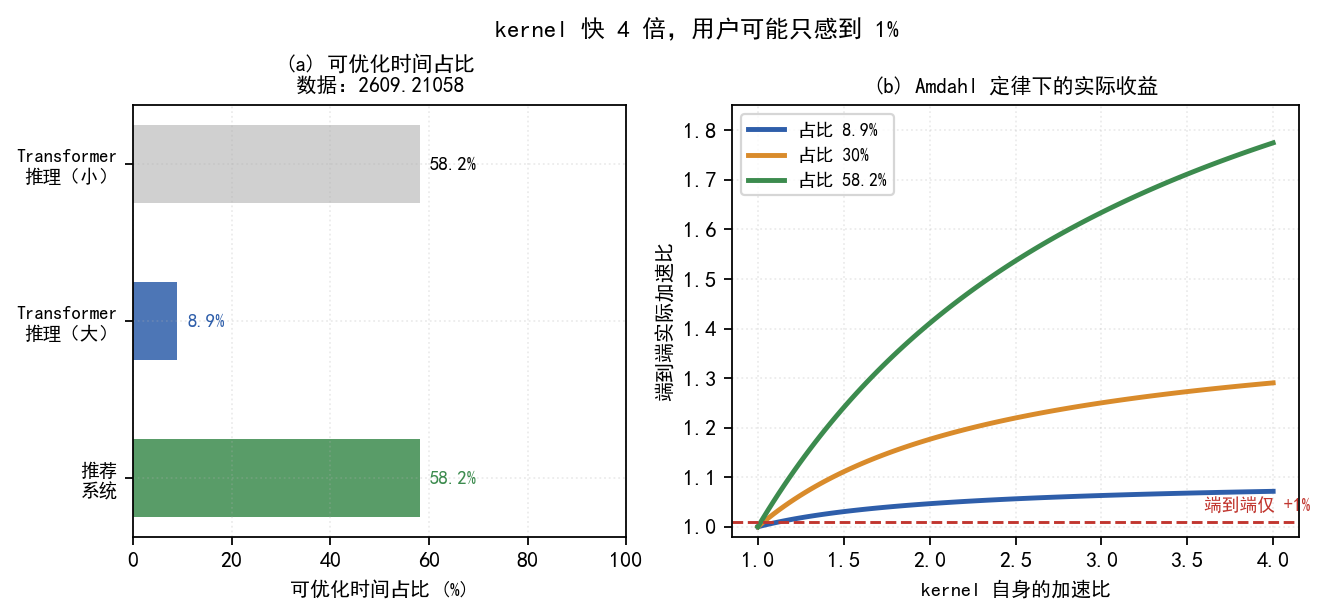
\includegraphics[width=0.86\textwidth]{../figures/fig9_endtoend.png}
\caption{kernel 加速与端到端收益的关系。(a) 真实负载中可优化时间的实测占比，数据来自 arXiv:2609.21058 的剖析；(b) 按 Amdahl 定律推算的端到端加速比，三条曲线对应不同可优化占比。在占比 8.9\% 的场景下，即使 kernel 本身快 4 倍，端到端也只有 1.07 倍。}
\label{fig:8}
\end{figure*}

\subsection{为什么这条结论重要}

这条发现重新定义了整个领域的价值定位。


\textbf{它不否定技术进步}。KernelBench 上的加速比是真实的，方法的演进也是真实的。但它指出：\textbf{benchmark 上的成功与生产环境的收益之间存在一个数量级的鸿沟}。


这个鸿沟有三个来源：


\begin{enumerate}
  \item \textbf{Amdahl 定律}。可优化部分占比小，整体提升必然受限。这是算术，不是意见。
  \item \textbf{被超越的对象是最强的部分}。GEMM 和 attention 是 cuBLAS/FlashAttention 的主场，而这些库由 NVIDIA 针对每代硬件手工调优。模型要赢的正是最难赢的地方。
  \item \textbf{规模效应反向}。模型越大，GEMM 占比越高，可优化空间越小。这意味着\textbf{这些方法在最需要性能的场景里最没用}。
\end{enumerate}

同一篇研究还顺手揭了 KernelBench 的一个底：它的正确性检查（\texttt{torch.allclose} 带绝对容差）在 \textbf{60 道 Level-1 题中有 4 道可以被全零张量通过}。也就是说，一个什么都不算的 kernel 能拿到 6.7\% 的「正确」分数{\scriptsize\texttt{c-\hspace{0pt}zero-\hspace{0pt}kernel}}。


\subsection{这解释了为什么工业界的采用是选择性的}

如果端到端收益只有 1\%，为什么还有公司在投入？


因为\textbf{场景差异极大}。推荐系统那 58.2\% 的可优化空间、集中在单个 embedding kernel 上——这种场景下 kernel 优化的回报是实打实的 8.63\%。同理，训练框架的核心算子、特定硬件的适配层、以及任何 cuBLAS 没有覆盖的算子，都是高价值目标。


所以正确的判断不是「这没用」，而是：\textbf{这是一个按场景定价的技术，而本领域几乎没有论文做这种定价。} 大家都在报「快了多少」，没人报「这值多少」。


本文认为这是当前最需要补上的一块。


\section{开放问题}

\subsection{性能层的诊断难题未解}

第 3 章指出性能层是真正的难题。至今没有工作能从根本上解决「如何从『慢』定位到『为什么慢』」。


现有做法依赖 profiler 提供硬件计数器，但这只是把问题往前推了一步：\textbf{计数器数值如何映射到具体的代码修改？} 这个映射关系本身就是专家知识的核心，也是 LLM 最难学到的部分。


一个可能的方向是把 kernel 优化知识显式化——不是让模型隐式学习，而是构建「症状 \sym{→}{} 原因 \sym{→}{} 修改」的知识库。但这又回到了「知识难以形式化」的原点。


2026 年 10 月的反思更进一步 [arXiv:2610.36576]：连「该 profile 什么」都不清楚。全量采集硬件计数器代价高昂，而多数计数器与当前瓶颈无关。他们的做法是\textbf{学习「少采集」}——用少量有判别力的指标替代全量剖析。这是把「诊断」从穷举转向定向的一步。


\subsection{可移植性几乎无人认真对待}

在 A100 上调优的 kernel，换到 H100 会怎样？现有工作大多只在单一硬件上评测。


CUDA-L1 提到了跨架构可移植性，KernelBenchX 专门测这个维度，但整体上这是被忽视的问题。而它对实际部署极为关键：企业的硬件是异构的，一个只在 H100 上快的 kernel 价值有限。


更深的问题是：\textbf{当模型「学会」了针对特定硬件的优化，它学到的是通用原理还是特定 trick？} 这个问题目前没有答案，但决定了这些方法的长期价值。


\subsection{正确性的保证强度不足}

现在的正确性依靠测试。测试通过不等于正确，只等于「在这些输入上对」。


Ave [arXiv:2604.18616] 的编译期不变量是一个正确方向——用类型系统式的约束保证变换合法。但要覆盖真实的 kernel 优化（涉及内存别名、竞态、浮点结合律），现有形式化方法远远不够。


一个务实的中期目标是：\textbf{对可验证的子集做强保证，其余部分靠测试 + 形式化的混合}。这需要明确划定「哪些优化是安全的」。


\subsection{成本与收益的边界未明}

Agent 与 RL 路线都需要大量搜索。CUDA Agent 的训练规模、KernelBlaster 的 MCTS 宽度，这些成本在论文中很少被完整报告。


一个关键但少有人问的问题是：\textbf{为了一个 1.2x 的加速，花 100 次 GPU 小时的搜索，值得吗？}


这取决于场景。对训练框架的核心算子（如 attention、GEMM），1.2x 意味着巨大的长期收益，值得。对一次性脚本，不值得。本领域缺少这种「按场景定价」的分析。


图 9 示意了收益递减的趋势。注意这是一张\textbf{示意}图，用于表达量级关系，不代表精确测量。


\begin{figure*}[t]
\centering
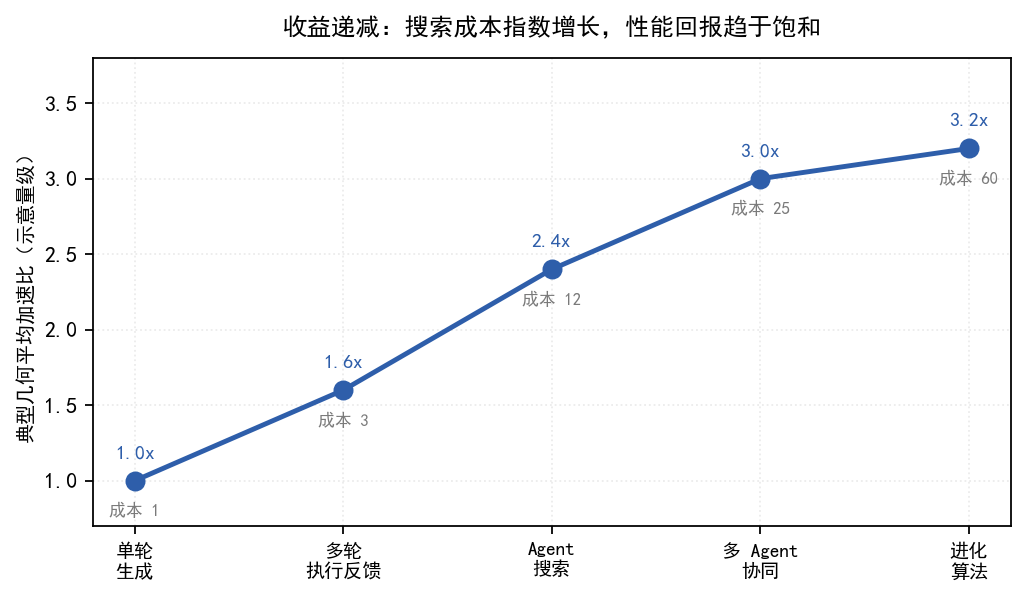
\includegraphics[width=0.86\textwidth]{../figures/fig7_tradeoff.png}
\caption{搜索成本与性能回报的收益递减关系。注意这是一张示意图，纵轴是量级估计而非实测值：横轴按系统复杂度排序（单轮生成 \sym{→}{} 多轮反馈 \sym{→}{} Agent 搜索 \sym{→}{} 多 Agent \sym{→}{} 进化算法），纵轴给出各路线典型几何平均加速比的大致位置，成本按相对倍数标注。要传达的是趋势：成本随复杂度呈指数增长，性能回报趋于饱和，提示「更多搜索」并非当前瓶颈的解法。}
\label{fig:9}
\end{figure*}

\subsection{评测的可持续性}

基准会饱和，也会被污染。KernelBench 的 250 题已在相当程度上被「刷过」，新基准（KernelBench-Verified、SOL-ExecBench）是回应。


但根本问题是：\textbf{评测框架与模型能力必须共同演进}。KernelBench-Verified 的结论「没有模型稳定超过 PyTorch」在当前是重要的纠偏，但它同样会随着模型进步而失效。


健康的做法是让基准\textbf{动态生成}——每次评测用新的、模型未见过的题目。这需要自动化的题目生成与验证流水线，目前尚不成熟。


\section{结论}

\subsection{主要发现}

\textbf{第一，这个领域在 18 个月内取得了实质进展，但幅度被系统性夸大。}


从「不到 20\% 的题目能打平 PyTorch」到「九成快于 \texttt{torch.compile}」，这是真实的进步。但当我们把基线校正到同等条件（TF32 + 隐藏测试），最强模型的几何平均回落到 0.88x——\textbf{尚未稳定超越 PyTorch}{\scriptsize\texttt{c-\hspace{0pt}kb-\hspace{0pt}baseline}}。


两个数字都对，只是回答的问题不同。\textbf{「进步的幅度」被高估了，但「进步的事实」成立。}


\textbf{第二，语法层与语义层已基本解决，性能层是唯一真正的难题。}


这个判断解释了方法演进：SFT 能解决语法与语义（模仿即可），但解决不了性能（相似度不等于速度）；RL 直接优化性能，但极易被奖励黑客；Agent 用搜索换性能，代价是成本。


\textbf{第三，度量危机是本领域当前最紧迫的问题。}


70 条速度声明中只有 11\% 可跨论文比较。基线漂移可造成 1.6 倍虚高，统计口径差异可造成 85 倍跨度。在这个基础上做「SOTA 竞争」，很大程度上是在比较不同的测量方法。


\subsection{对实践者的建议}

\textbf{如果你要选用这些工具}：优先看它报告的是几何平均还是 up-to，基线是否明确开了 TF32，是否有隐藏测试集结果。三个问题能过滤掉大部分夸大。


\textbf{如果你要做这个方向的研究}：报告三元组（几何平均/中位数/优于基线比例），明确基线配置，报告失败率与显存。这三件事的成本很低，但对领域健康的价值很高。


\textbf{如果你要评估一篇论文的可信度}：看它是否讨论了自己的失败案例。本领域中，坦率报告「我们的方法在 X 类算子上无效」的论文，往往比只报最好数字的更可靠。


\subsection{一句话总结}

\begin{quote}\small
\textbf{CUDA kernel 生成已经解决了「写得出来」，正在解决「写得快」，而「快」这个标准本身还没有被可靠地测量。}

\end{quote}

\section{附录 A　论文清单}

本文纳入的 98 篇论文按时间排列，完整元数据见 \texttt{papers.json}。以下列出方法谱系中的 15 篇核心工作。


\begin{table*}[t]
\centering
\footnotesize
\setlength{\tabcolsep}{4pt}
\caption{方法谱系中的 15 篇核心工作}
\label{tab:12}
\begin{tabular}{llll}
\toprule
路线 & 系统 & arXiv & 核心机制 \\
\midrule
SFT & KernelLLM & HF 模型卡 & Llama-3.1-8B 微调 \\
SFT & ConCuR & 2510.07356 & 精简推理链 \\
SFT & Tokens to Regions & 2606.16231 & 区域级指令微调 \\
RL & Kevin & 2507.11948 & 多轮 RL \\
RL & CUDA-L1 & 2507.14111 & 对比式 RL \\
RL & AutoTriton & 2507.05687 & Triton + RL \\
RL & QiMeng-Kernel & 2511.20100 & 宏观思考/微观编码 \\
RL & CUDA-L2 & 2512.02551 & 执行速度奖励 \\
RL & Dr. Kernel & 2602.05885 & TRLOO 去偏 \\
RL & CUDA Agent & 2602.24286 & 大规模 Agentic RL \\
Agent & GPU Kernel Scientist & 2506.20807 & 进化式 Agent \\
Agent & STARK & 2510.16996 & 多 Agent 协同 \\
Agent & CudaForge & 2511.01884 & 硬件反馈 \\
Agent & KernelBlaster & 2602.14293 & MCTS 搜索 \\
Agent & Ave & 2604.18616 & 数据流不变量 \\
\bottomrule
\end{tabular}
\end{table*}



\section{附录 B　基准对比}

\begin{table*}[t]
\centering
\footnotesize
\setlength{\tabcolsep}{4pt}
\caption{主流基准对比}
\label{tab:13}
\begin{tabular}{lrrrll}
\toprule
基准 & arXiv & 时间 & 题目数 & 基线 & 主指标 \\
\midrule
KernelBench & 2502.10517 & 2025-02 & 250 & PyTorch & fast\_p \\
TritonBench & 2502.14752 & 2025-02 & 184 & PyTorch/Triton & 正确性+加速比 \\
MultiKernelBench & 2507.17773 & 2025-07 & 285 & PyTorch & pass@k+加速比 \\
KernelBench-Verified & 2607.16241 & 2026-06 & 250 & TF32 PyTorch & 几何平均+内存 \\
KernelBenchX & 2605.04956 & 2026-05 & — & PyTorch/Triton & 可移植性 \\
SOL-ExecBench & 2603.19173 & 2026-03 & — & 硬件上限 & 达上限比例 \\
\bottomrule
\end{tabular}
\end{table*}



\section{附录 C　可复现性说明}

本文全部分析可由以下脚本重跑：


\begin{lstlisting}
python fetch_papers.py       # 抓取 98 篇 arXiv 元数据 -> papers.json
python extract_metrics.py    # 抽取量化指标 -> extracted.json
python classify_claims.py    # 分类速度声明 -> speed_claims.json
python make_figures.py       # 生成 7 张图 -> figures/
python make_tables.py        # 生成 5 张表 -> tables/
\end{lstlisting}

\textbf{数据来源}：arXiv 官方 API（\texttt{export.arxiv.org/api/query}），非二手转述。


\textbf{已知局限}：


\begin{enumerate}
  \item 定量分析基于摘要而非全文（第 1.4 节已说明）
  \item 70 条速度声明来自正则抽取，可能漏掉非标准表述
  \item 「可跨论文比较的 8 条」是保守下界——有些论文可能在其他章节报告了严格数字
\end{enumerate}

\textbf{校验}：\texttt{make\_tables.py} 内置回溯检查，把表 7 的每个数值回查 \texttt{papers.json} 的摘要原文，找不到即报错。当前全部通过。

